\documentclass[12pt]{article}
\usepackage[utf8]{inputenc}
\usepackage[T1]{fontenc}
\usepackage[margin=1in,headheight=15pt]{geometry}
\usepackage{amsmath,amssymb}
\usepackage{lmodern}
\usepackage{xcolor}
\usepackage[most]{tcolorbox}
\usepackage{enumitem}
\usepackage{fancyhdr}
\usepackage{booktabs}
\usepackage{array}
\usepackage{tikz}

%-- Colors
\definecolor{navy}{RGB}{0,32,96}
\definecolor{crimson}{RGB}{180,0,0}
\definecolor{darkgreen}{RGB}{0,100,0}
\definecolor{teal}{RGB}{0,100,120}
\definecolor{orange}{RGB}{200,80,0}
\definecolor{bgblue}{RGB}{235,242,255}
\definecolor{bggreen}{RGB}{235,255,240}
\definecolor{bgyellow}{RGB}{255,252,225}
\definecolor{bgred}{RGB}{255,235,235}
\definecolor{bgorange}{RGB}{255,245,225}
\definecolor{bgteal}{RGB}{230,248,250}
\definecolor{bgpurple}{RGB}{245,235,255}
\definecolor{purple}{RGB}{90,0,150}

%-- Header
\pagestyle{fancy}
\fancyhf{}
\lhead{\textbf{Chapter 8}\quad\textit{nth Roots \& Rational Exponents --- Complete Guide}}
\rhead{\textit{Algebra 1}}
\cfoot{\thepage}
\renewcommand{\headrulewidth}{0.5pt}

%-- Section counter
\newcounter{mysec}
\newcommand{\mysection}[1]{%
  \stepcounter{mysec}%
  \vspace{14pt}%
  \noindent
  \begin{tcolorbox}[enhanced,colback=navy,colframe=navy,
    boxrule=0pt,arc=3pt,left=8pt,right=8pt,top=5pt,bottom=5pt,
    before skip=0pt,after skip=10pt]
    \color{white}\bfseries\large Section~\themysec\enspace---\enspace #1
  \end{tcolorbox}}

%-- Boxes
\newtcolorbox{insightbox}[1]{enhanced,breakable,
  colback=bgorange,colframe=orange,
  title={\textbf{#1}},fonttitle=\bfseries\color{white},
  attach boxed title to top left={yshift=-2mm,xshift=6mm},
  boxed title style={colback=orange,colframe=orange,arc=2pt},
  arc=3pt,left=8pt,right=8pt,top=10pt,bottom=8pt,
  before skip=6pt,after skip=10pt}

\newtcolorbox{conceptbox}[1]{enhanced,breakable,
  colback=bgblue,colframe=navy,
  title={\textbf{Core Concept: }#1},fonttitle=\bfseries\color{white},
  attach boxed title to top left={yshift=-2mm,xshift=6mm},
  boxed title style={colback=navy,colframe=navy,arc=2pt},
  arc=3pt,left=8pt,right=8pt,top=10pt,bottom=8pt,
  before skip=6pt,after skip=10pt}

\newtcolorbox{bigpicturebox}{enhanced,breakable,
  colback=bggreen,colframe=darkgreen,
  title={\textbf{The Big Picture}},fonttitle=\bfseries\color{white},
  attach boxed title to top left={yshift=-2mm,xshift=6mm},
  boxed title style={colback=darkgreen,colframe=darkgreen,arc=2pt},
  arc=3pt,left=8pt,right=8pt,top=10pt,bottom=8pt,
  before skip=6pt,after skip=10pt}

\newtcolorbox{examplebox}[1]{enhanced,breakable,
  colback=bggreen,colframe=darkgreen,
  title={\textbf{Worked Example: }#1},fonttitle=\bfseries\color{white},
  attach boxed title to top left={yshift=-2mm,xshift=6mm},
  boxed title style={colback=darkgreen,colframe=darkgreen,arc=2pt},
  arc=3pt,left=8pt,right=8pt,top=10pt,bottom=8pt,
  before skip=6pt,after skip=10pt}

\newtcolorbox{practicebox}[1]{enhanced,breakable,
  colback=bgyellow,colframe=crimson,
  title={\textbf{#1}},fonttitle=\bfseries\color{white},
  attach boxed title to top left={yshift=-2mm,xshift=6mm},
  boxed title style={colback=crimson,colframe=crimson,arc=2pt},
  arc=3pt,left=8pt,right=8pt,top=10pt,bottom=8pt,
  before skip=6pt,after skip=10pt}

\newtcolorbox{solutionbox}[1]{enhanced,breakable,
  colback=bgred,colframe=crimson,
  title={\textbf{#1}},fonttitle=\bfseries\color{white},
  attach boxed title to top left={yshift=-2mm,xshift=6mm},
  boxed title style={colback=crimson,colframe=crimson,arc=2pt},
  arc=3pt,left=8pt,right=8pt,top=10pt,bottom=8pt,
  before skip=6pt,after skip=14pt}

\newtcolorbox{notebox}{enhanced,
  colback=bgteal,colframe=teal,
  arc=3pt,left=8pt,right=8pt,top=6pt,bottom=6pt,
  before skip=6pt,after skip=8pt}

\newtcolorbox{tipbox}{enhanced,
  colback=bgpurple,colframe=purple,
  arc=3pt,left=8pt,right=8pt,top=6pt,bottom=6pt,
  before skip=6pt,after skip=8pt}

\newcommand{\step}[1]{\hfill\textcolor{crimson}{\small\textit{#1}}}

\begin{document}

%======================================================
%  TITLE
%======================================================
\begin{tcolorbox}[enhanced,colback=navy,colframe=navy,arc=6pt,
  left=12pt,right=12pt,top=12pt,bottom=12pt]
  \centering\color{white}
  {\LARGE\bfseries Chapter 8 --- nth Roots \& Rational Exponents}\\[6pt]
  {\large Algebra 1 \quad $\bullet$ \quad Complete Study Guide: Concept to Practice}
\end{tcolorbox}

\vspace{6pt}
\noindent\textbf{What You Will Learn:}\;
(1)~Where radical notation comes from.\;
(2)~Find $n$th roots and understand the four cases.\;
(3)~Evaluate and simplify rational exponents.\;
(4)~Apply exponent properties.\;
(5)~Solve real-life problems.

\vspace{4pt}\hrule\vspace{8pt}

%======================================================
% SECTION 1 --- WHY RADICALS EXIST (Motivation)
%======================================================
\mysection{Where Does the Radical Sign Come From?}

\begin{insightbox}{Key Insight: Radicals Are Like Long Division}
The radical sign $\sqrt{\phantom{x}}$ grew out of the idea of \textbf{long division}!
Just as long division \textit{undoes} multiplication,
taking a root \textit{undoes} exponentiation.
\end{insightbox}

\noindent\textbf{Step 1 --- Start with multiplication:}
\[
  6 = 2 \times 3
\]

\noindent\textbf{Step 2 --- Division undoes it:}
\[
  2\,\overline{\big)\,6} \quad\Rightarrow\quad 3
\]

\noindent\textbf{Step 3 --- Scale up to exponentiation:}
\[
  \underbrace{a \cdot a \cdot a \cdots a}_{10\text{ times}} = 1024
  \qquad\Longrightarrow\qquad
  \sqrt[10]{1024} = a = 2
\]

\begin{center}
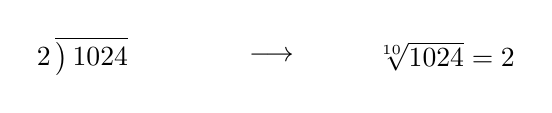
\begin{tikzpicture}
  \node at (0,0) {$2\,\overline{\big)\,1024}$};
  \node at (2.4,0) {$\longrightarrow$};
  \node at (4.6,0) {$\sqrt[10]{1024}=2$};
\end{tikzpicture}
\end{center}

\begin{center}
\renewcommand{\arraystretch}{1.4}
\begin{tabular}{ccc}
\toprule
\textbf{Operation} & \textbf{Symbol} & \textbf{Meaning} \\
\midrule
Multiplication  & $2\times3=6$          & Combine equal groups \\
Long Division   & $2\,\overline{\big)\,6}$ & \textbf{Undo} multiplication \\
Exponentiation  & $2^{10}=1024$         & Repeated multiplication \\
Radical         & $\sqrt[10]{1024}=2$   & \textbf{Undo} exponentiation \\
\bottomrule
\end{tabular}
\end{center}

\begin{bigpicturebox}
Three operations --- same relationship, different unknown:
\[
  \underbrace{b^{\,p}=x}_{\text{exponentiation: find }x}
  \;\iff\;
  \underbrace{b=\sqrt[p]{x}}_{\text{radical: find }b}
  \;\iff\;
  \underbrace{p=\log_b x}_{\text{logarithm: find }p}
\]
\textbf{Exponentiation, radicals, and logarithms are the same triangle of ideas.}
\end{bigpicturebox}

%======================================================
% SECTION 2 --- CORE DEFINITION
%======================================================
\mysection{Core Definition of Rational Exponents}

\begin{conceptbox}{The Key Formula}
\[
  \boxed{a^{m/n} \;=\; \sqrt[n]{a^m} \;=\; \Bigl(\sqrt[n]{a}\Bigr)^m}
\]
\begin{center}
\large\textbf{Denominator} of the exponent $=$ the \textbf{Root index}\\[4pt]
\textbf{Numerator} of the exponent $=$ the \textbf{Power}
\end{center}

\medskip
Special case ($m=1$):\quad $a^{1/n}=\sqrt[n]{a}$
\end{conceptbox}

\noindent Connection to rational exponents via the Power of a Power property:
\[
  (a^{1/2})^2 = a^{(1/2)\cdot2}=a^1=a, \quad
  (a^{1/3})^3 = a^1=a, \quad
  (a^{1/4})^4 = a^1=a
\]
Therefore $a^{1/n}$ \emph{is} the $n$th root of $a$.

%======================================================
% SECTION 3 --- FINDING nth ROOTS (Four Cases)
%======================================================
\mysection{Finding \textit{n}th Roots --- The Four Cases}

\begin{conceptbox}{Real \textit{n}th Roots of $a$}
Let $n>1$ be an integer and $a$ a real number.
\begin{center}
\renewcommand{\arraystretch}{1.5}
\begin{tabular}{@{}llll@{}}
\toprule
\textbf{Condition} & \textbf{Real roots} & \textbf{Count} & \textbf{Example} \\
\midrule
$n$ \textbf{odd}, any $a$       & $\sqrt[n]{a}$       & One   & $\sqrt[3]{-8}=-2$ \\
$n$ \textbf{even}, $a>0$        & $\pm\sqrt[n]{a}$    & Two   & $\pm\sqrt[4]{16}=\pm2$ \\
$n$ \textbf{even}, $a=0$        & $0$                 & One   & $\sqrt[4]{0}=0$ \\
$n$ \textbf{even}, $a<0$        & (none)              & Zero  & $\sqrt[4]{-16}$ undefined \\
\bottomrule
\end{tabular}
\end{center}
\begin{notebox}
$\pm\sqrt[n]{a}$ represents \emph{both} the positive and negative $n$th roots.
An even index with a negative radicand produces \textbf{no real number}.
\end{notebox}
\end{conceptbox}

\begin{examplebox}{Identifying and Finding nth Roots}
Find each root, or state if not a real number.\\[4pt]
\textbf{(a)}~$\sqrt[3]{27}$\quad
\textbf{(b)}~$\sqrt[3]{-64}$\quad
\textbf{(c)}~$\pm\sqrt[4]{625}$\quad
\textbf{(d)}~$\sqrt[4]{-81}$\quad
\textbf{(e)}~$\sqrt[5]{-243}$
\tcblower
\textbf{(a)} $\sqrt[3]{27}=\sqrt[3]{3^3}=3$ \step{odd index, positive radicand}

\medskip
\textbf{(b)} $\sqrt[3]{-64}=\sqrt[3]{(-4)^3}=-4$ \step{odd index allows negative radicand}

\medskip
\textbf{(c)} $\pm\sqrt[4]{625}=\pm\sqrt[4]{5^4}=\pm5$ \step{even index, $a>0$: two roots}

\medskip
\textbf{(d)} $\sqrt[4]{-81}$ is \textbf{not a real number} \step{even index, $a<0$}

\medskip
\textbf{(e)} $\sqrt[5]{-243}=\sqrt[5]{(-3)^5}=-3$ \step{odd index: one real root}
\end{examplebox}

%======================================================
% SECTION 4 --- EVALUATING a^(1/n)
%======================================================
\mysection{Evaluating Expressions of the Form $a^{1/n}$}

\begin{conceptbox}{Key Distinction: Where Is the Negative Sign?}
\begin{center}
\renewcommand{\arraystretch}{1.5}
\begin{tabular}{@{}lll@{}}
\toprule
\textbf{Expression} & \textbf{Meaning} & \textbf{Value} \\
\midrule
$8^{1/3}$        & $\sqrt[3]{8}$          & $2$ \\
$(-8)^{1/3}$     & $\sqrt[3]{-8}$         & $-2$ \quad (odd index: OK) \\
$-8^{1/3}$       & $-(\sqrt[3]{8})$       & $-2$ \quad (negate after rooting) \\
$(-16)^{1/4}$    & $\sqrt[4]{-16}$        & \textit{not real} \quad (even index, $a<0$) \\
$-16^{1/4}$      & $-(\sqrt[4]{16})$      & $-2$ \quad (negate after rooting) \\
\bottomrule
\end{tabular}
\end{center}
\end{conceptbox}

\begin{examplebox}{Evaluating $a^{1/n}$ --- Sign Placement}
\textbf{(a)}~$(-8)^{1/3}$\quad \textbf{(b)}~$-\!\sqrt[3]{8}$\quad
\textbf{(c)}~$16^{1/4}$\quad \textbf{(d)}~$(-16)^{1/4}$
\tcblower
\textbf{(a)} $(-8)^{1/3}=\sqrt[3]{(-2)^3}=-2$ \step{odd index; root of a negative number}

\medskip
\textbf{(b)} $-\!\sqrt[3]{8}=-(\sqrt[3]{2^3})=-2$ \step{negate the principal root}

\medskip
\textbf{(c)} $16^{1/4}=\sqrt[4]{2^4}=2$ \step{positive principal fourth root}

\medskip
\textbf{(d)} $(-16)^{1/4}$ is \textbf{not a real number} \step{even index with negative base}
\end{examplebox}

%======================================================
% SECTION 5 --- TWO METHODS FOR a^(m/n)
%======================================================
\mysection{Evaluating $a^{m/n}$ --- Two Methods}

\begin{conceptbox}{Root First vs.\ Power First}
\[
  a^{m/n} = \Bigl(\sqrt[n]{a}\Bigr)^m \quad\textbf{(Method 1: root first)}
  \qquad=\qquad
  \sqrt[n]{a^m} \quad\textbf{(Method 2: power first)}
\]
\begin{center}
\renewcommand{\arraystretch}{1.5}
\begin{tabular}{>{\bfseries}ccc}
\toprule
Expression & Method 1: Root First & Method 2: Power First \\
\midrule
$8^{2/3}$
  & $(\sqrt[3]{8})^2=2^2=4$
  & $\sqrt[3]{8^2}=\sqrt[3]{64}=4$ \\[4pt]
$16^{3/4}$
  & $(\sqrt[4]{16})^3=2^3=8$
  & $\sqrt[4]{16^3}=\sqrt[4]{4096}=8$ \\
\bottomrule
\end{tabular}
\end{center}
\begin{tipbox}
\textbf{Tip:} Root first is almost always easier --- it keeps numbers small before you raise to a power.
\end{tipbox}
\end{conceptbox}

\begin{examplebox}{Full Set of Worked Examples}
\textbf{(1)}~$9^{1/2}$\quad
\textbf{(2)}~$27^{2/3}$\quad
\textbf{(3)}~$32^{3/5}$\quad
\textbf{(4)}~$(-8)^{2/3}$\quad
\textbf{(5)}~$4^{-3/2}$\quad
\textbf{(6)}~$\left(\dfrac{4}{9}\right)^{3/2}$\quad
\textbf{(7)}~$(-27)^{2/3}$\quad
\textbf{(8)}~$81^{-3/4}$
\tcblower
\textbf{(1)} $9^{1/2}=\sqrt{9}=\boxed{3}$ \step{square root}

\medskip
\textbf{(2)} $27^{2/3}=(\sqrt[3]{27})^2=3^2=\boxed{9}$ \step{cube root first, then square}

\medskip
\textbf{(3)} $32^{3/5}=(\sqrt[5]{32})^3=2^3=\boxed{8}$ \step{fifth root first, then cube}

\medskip
\textbf{(4)} $(-8)^{2/3}=(\sqrt[3]{-8})^2=(-2)^2=\boxed{4}$ \step{odd index allows negative base}

\medskip
\textbf{(5)} $4^{-3/2}=\dfrac{1}{4^{3/2}}=\dfrac{1}{(\sqrt{4})^3}=\dfrac{1}{2^3}=\boxed{\dfrac{1}{8}}$ \step{negative exponent $\Rightarrow$ reciprocal}

\medskip
\textbf{(6)} $\left(\dfrac{4}{9}\right)^{3/2}=\left(\sqrt{\dfrac{4}{9}}\right)^3=\left(\dfrac{2}{3}\right)^3=\boxed{\dfrac{8}{27}}$ \step{root the fraction, then cube}

\medskip
\textbf{(7)} $(-27)^{2/3}=(\sqrt[3]{-27})^2=(-3)^2=\boxed{9}$ \step{odd index; squaring makes positive}

\medskip
\textbf{(8)} $81^{-3/4}=\dfrac{1}{81^{3/4}}=\dfrac{1}{(\sqrt[4]{81})^3}=\dfrac{1}{3^3}=\boxed{\dfrac{1}{27}}$ \step{reciprocal, then root first}
\end{examplebox}

%======================================================
% SECTION 6 --- NEGATIVE RATIONAL EXPONENTS
%======================================================
\mysection{Negative Rational Exponents}

\begin{conceptbox}{Negative Exponent Rule}
\[
  \boxed{a^{-m/n} = \frac{1}{a^{m/n}}}, \qquad a \neq 0
\]
\textbf{Strategy:} flip to reciprocal first, then evaluate $a^{m/n}$ as usual.

\medskip
\textbf{Example:}\quad
$27^{-2/3}
=\dfrac{1}{27^{2/3}}
=\dfrac{1}{(\sqrt[3]{27})^2}
=\dfrac{1}{3^2}
=\dfrac{1}{9}$
\end{conceptbox}

%======================================================
% SECTION 7 --- EXPONENT PROPERTIES
%======================================================
\mysection{Exponent Properties with Rational Exponents}

\begin{conceptbox}{All Five Laws Still Apply}
\begin{center}
\renewcommand{\arraystretch}{1.6}
\begin{tabular}{@{}lll@{}}
\toprule
\textbf{Property} & \textbf{Rule} & \textbf{Example} \\
\midrule
Product of powers  & $a^m\cdot a^n=a^{m+n}$
  & $8^{1/3}\cdot8^{2/3}=8^1=8$ \\
Quotient of powers & $\dfrac{a^m}{a^n}=a^{m-n}$
  & $\dfrac{16^{3/4}}{16^{1/4}}=16^{1/2}=4$ \\
Power of a power   & $(a^m)^n=a^{mn}$
  & $(9^{1/2})^4=9^2=81$ \\
Power of a product & $(ab)^m=a^m b^m$
  & $(4\cdot9)^{1/2}=2\cdot3=6$ \\
Power of a quotient& $\left(\dfrac{a}{b}\right)^m=\dfrac{a^m}{b^m}$
  & $\left(\dfrac{8}{27}\right)^{1/3}=\dfrac{2}{3}$ \\
\bottomrule
\end{tabular}
\end{center}
\end{conceptbox}

\begin{examplebox}{Simplifying with Exponent Properties}
\textbf{(a)}~$5^{1/3}\cdot5^{2/3}$\quad
\textbf{(b)}~$\dfrac{x^{3/4}}{x^{1/4}}$\quad
\textbf{(c)}~$(x^{2/3})^{3/2}$\quad
\textbf{(d)}~$\left(\dfrac{27}{8}\right)^{2/3}$
\tcblower
\textbf{(a)} $5^{1/3}\cdot5^{2/3}=5^{1/3+2/3}=5^1=5$ \step{product of powers}

\medskip
\textbf{(b)} $\dfrac{x^{3/4}}{x^{1/4}}=x^{3/4-1/4}=x^{1/2}$ \step{quotient of powers}

\medskip
\textbf{(c)} $(x^{2/3})^{3/2}=x^{(2/3)(3/2)}=x^1=x$ \step{power of a power}

\medskip
\textbf{(d)} $\left(\dfrac{27}{8}\right)^{2/3}=\dfrac{27^{2/3}}{8^{2/3}}=\dfrac{3^2}{2^2}=\dfrac{9}{4}$ \step{power of a quotient, then root first}
\end{examplebox}

%======================================================
% SECTION 8 --- CONVERTING FORMS
%======================================================
\mysection{Converting Between Radical and Exponential Forms}

\begin{conceptbox}{Conversion at a Glance}
\[
  \sqrt[n]{a^m} = a^{m/n}
  \qquad\longleftrightarrow\qquad
  a^{m/n} = \sqrt[n]{a^m}
\]
\begin{center}
\renewcommand{\arraystretch}{1.4}
\begin{tabular}{@{}ll@{}}
\toprule
Radical form & Exponential form \\
\midrule
$\sqrt[3]{x^2}$ & $x^{2/3}$ \\
$(\sqrt[4]{z})^3$ & $z^{3/4}$ \\
$\dfrac{1}{\sqrt[3]{a^2}}$ & $a^{-2/3}$ \\
$\sqrt[3]{x^6}$ & $x^{6/3}=x^2$ \\
\bottomrule
\end{tabular}
\end{center}
\end{conceptbox}

\begin{examplebox}{Converting Forms}
\textbf{(a)} Write $\sqrt[4]{x^3}$ in exponential form.\\
\textbf{(b)} Write $a^{5/6}$ in radical form.\\
\textbf{(c)} Write $\dfrac{1}{\sqrt[3]{y^4}}$ with a rational exponent.\\
\textbf{(d)} Simplify $\sqrt[3]{x^6}$.
\tcblower
\textbf{(a)} $\sqrt[4]{x^3}=x^{3/4}$ \step{index $\to$ denominator, power $\to$ numerator}

\medskip
\textbf{(b)} $a^{5/6}=\sqrt[6]{a^5}$ \step{denominator is index, numerator is power}

\medskip
\textbf{(c)} $\dfrac{1}{\sqrt[3]{y^4}}=\dfrac{1}{y^{4/3}}=y^{-4/3}$ \step{reciprocal gives negative exponent}

\medskip
\textbf{(d)} $\sqrt[3]{x^6}=x^{6/3}=x^2$ \step{convert, simplify the fraction}
\end{examplebox}

%======================================================
% SECTION 9 --- PRACTICE PROBLEMS (Three Levels)
%======================================================
\mysection{Practice Problems}

\begin{practicebox}{Level 1 --- Evaluate (nth Roots and $a^{1/n}$)}
\begin{enumerate}[label=\textbf{\arabic*.},leftmargin=*,itemsep=8pt]
  \item $\sqrt[3]{125}$
  \item $\sqrt[3]{-216}$
  \item $\pm\sqrt[4]{256}$
  \item $\sqrt[6]{-64}$
  \item $64^{1/3}$\quad (write as a radical first)
  \item $25^{3/2}$
  \item $81^{3/4}$
  \item $(-32)^{1/5}$
\end{enumerate}
\end{practicebox}

\begin{practicebox}{Level 2 --- Negative Exponents and Mixed Forms}
\begin{enumerate}[label=\textbf{\arabic*.},leftmargin=*,itemsep=8pt]
  \item $16^{-1/4}$
  \item $8^{-2/3}$
  \item $27^{-4/3}$
  \item $81^{-3/4}$
  \item $(-32)^{3/5}$
  \item $\left(\dfrac{4}{9}\right)^{3/2}$
  \item $\left(\dfrac{8}{27}\right)^{2/3}$
  \item $(-8)^{4/3}$
\end{enumerate}
\end{practicebox}

\begin{practicebox}{Level 3 --- Exponent Properties and Conversion}
\begin{enumerate}[label=\textbf{\arabic*.},leftmargin=*,itemsep=8pt]
  \item $8^{1/3}\cdot8^{2/3}$
  \item $\dfrac{16^{3/4}}{16^{1/4}}$
  \item $4^{1/2}\cdot9^{1/2}$
  \item $(9^{1/2})^4$
  \item $7^{1/4}\cdot7^{3/4}$
  \item $\dfrac{x^{5/6}}{x^{1/6}}$ \quad(simplify)
  \item $(y^{3/4})^{8/3}$ \quad(simplify)
  \item $\left(\dfrac{64}{125}\right)^{2/3}$
\end{enumerate}
\end{practicebox}

\begin{practicebox}{Level 4 --- Converting Forms and Solving Equations}
\begin{enumerate}[label=\textbf{\arabic*.},leftmargin=*,itemsep=8pt]
  \item Write $\sqrt[5]{m^3}$ in exponential form.
  \item Write $(\sqrt[4]{p})^7$ in exponential form.
  \item Write $\dfrac{1}{\sqrt[6]{k^5}}$ using a rational exponent.
  \item Evaluate $125^{2/3}$ by rewriting in radical form first.
  \item Evaluate $243^{3/5}$ by rewriting in radical form first.
  \item Solve for $x$:\; $x^{3/4}=27$
  \item Solve for $x$:\; $x^{2/3}=16$
  \item Solve for $x$:\; $x^{-1/2}=\dfrac{1}{3}$
\end{enumerate}
\end{practicebox}

%======================================================
% SECTION 10 --- REAL-LIFE APPLICATIONS
%======================================================
\mysection{Real-Life Applications}

\begin{conceptbox}{Strategy}
\begin{enumerate}
  \item Write the formula and identify the variable with a rational exponent.
  \item Raise both sides to the \textbf{reciprocal} exponent to isolate the variable.
  \item Simplify and check that the answer makes sense in context.
\end{enumerate}
\end{conceptbox}

\begin{examplebox}{Real-Life Problems}
\textbf{(a)} \textit{Geometry:} The edge of a cube with volume $V$ is $s=V^{1/3}$.
Find $s$ when $V=343\text{ cm}^3$.

\medskip
\textbf{(b)} \textit{Physics:} Pendulum period $T=2\pi\!\left(\dfrac{L}{9.8}\right)^{1/2}$ s.
Find $T$ when $L=2.45$ m.
\tcblower
\textbf{(a)} $s=343^{1/3}=\sqrt[3]{7^3}=7\text{ cm}$ \step{cube root}

\medskip
\textbf{(b)}
\[
  T=2\pi\!\left(\tfrac{2.45}{9.8}\right)^{1/2}=2\pi(0.25)^{1/2}=2\pi(0.5)=\pi\approx3.1\text{ s}
\]
\end{examplebox}

\begin{practicebox}{Level 5 --- Real-Life Problems}
\begin{enumerate}[label=\textbf{\arabic*.},leftmargin=*,itemsep=12pt]
  \item A cube has volume $512\text{ in}^3$. Find its edge length using $s=V^{1/3}$.
  \item The radius of a sphere: $r=\left(\dfrac{3V}{4\pi}\right)^{1/3}$.
    Find $r$ when $V=\dfrac{4\pi}{3}$ cubic units.
  \item Skid-mark speed: $v=(24d)^{1/2}$ mph. Find $v$ when $d=6$ ft.
  \item Solve: $x^{3/4}=27$.
  \item Solve: $x^{2/3}=16$.
\end{enumerate}
\end{practicebox}

%======================================================
%  COMPLETE SOLUTIONS
%======================================================
\newpage
\begin{tcolorbox}[enhanced,colback=navy,colframe=navy,arc=6pt,
  left=12pt,right=12pt,top=8pt,bottom=8pt]
  \centering\color{white}{\Large\bfseries Complete Solutions --- Chapter 8}
\end{tcolorbox}
\vspace{8pt}

\begin{solutionbox}{Level 1 --- nth Roots and $a^{1/n}$}
\textbf{1.}~$\sqrt[3]{125}=5$\quad
\textbf{2.}~$\sqrt[3]{-216}=-6$\quad
\textbf{3.}~$\pm\sqrt[4]{256}=\pm4$\quad
\textbf{4.}~Not a real number (even index, $a<0$)

\medskip
\textbf{5.}~$64^{1/3}=\sqrt[3]{64}=4$\quad
\textbf{6.}~$25^{3/2}=(\sqrt{25})^3=5^3=125$\quad
\textbf{7.}~$81^{3/4}=(\sqrt[4]{81})^3=3^3=27$\quad
\textbf{8.}~$(-32)^{1/5}=-2$
\end{solutionbox}

\begin{solutionbox}{Level 2 --- Negative Exponents and Mixed Forms}
\textbf{1.}~$16^{-1/4}=\dfrac{1}{\sqrt[4]{16}}=\dfrac{1}{2}$\quad
\textbf{2.}~$8^{-2/3}=\dfrac{1}{(\sqrt[3]{8})^2}=\dfrac{1}{4}$\quad
\textbf{3.}~$27^{-4/3}=\dfrac{1}{(\sqrt[3]{27})^4}=\dfrac{1}{81}$

\medskip
\textbf{4.}~$81^{-3/4}=\dfrac{1}{(\sqrt[4]{81})^3}=\dfrac{1}{27}$\quad
\textbf{5.}~$(-32)^{3/5}=(\sqrt[5]{-32})^3=(-2)^3=-8$

\medskip
\textbf{6.}~$\left(\dfrac{4}{9}\right)^{3/2}=\left(\dfrac{2}{3}\right)^3=\dfrac{8}{27}$\quad
\textbf{7.}~$\left(\dfrac{8}{27}\right)^{2/3}=\dfrac{(\sqrt[3]{8})^2}{(\sqrt[3]{27})^2}=\dfrac{4}{9}$\quad
\textbf{8.}~$(-8)^{4/3}=(\sqrt[3]{-8})^4=(-2)^4=16$
\end{solutionbox}

\begin{solutionbox}{Level 3 --- Exponent Properties}
\textbf{1.}~$8^{1/3}\cdot8^{2/3}=8^1=8$\quad
\textbf{2.}~$\dfrac{16^{3/4}}{16^{1/4}}=16^{1/2}=4$\quad
\textbf{3.}~$4^{1/2}\cdot9^{1/2}=(36)^{1/2}=6$\quad
\textbf{4.}~$(9^{1/2})^4=9^2=81$

\medskip
\textbf{5.}~$7^{1/4}\cdot7^{3/4}=7^1=7$\quad
\textbf{6.}~$\dfrac{x^{5/6}}{x^{1/6}}=x^{4/6}=x^{2/3}$\quad
\textbf{7.}~$(y^{3/4})^{8/3}=y^2$\quad
\textbf{8.}~$\left(\dfrac{64}{125}\right)^{2/3}=\dfrac{16}{25}$
\end{solutionbox}

\begin{solutionbox}{Level 4 --- Converting and Solving}
\textbf{1.}~$m^{3/5}$\quad
\textbf{2.}~$p^{7/4}$\quad
\textbf{3.}~$k^{-5/6}$

\medskip
\textbf{4.}~$125^{2/3}=(\sqrt[3]{125})^2=5^2=25$\quad
\textbf{5.}~$243^{3/5}=(\sqrt[5]{243})^3=3^3=27$

\medskip
\textbf{6.}~$x^{3/4}=27\;\Rightarrow\;x=27^{4/3}=(\sqrt[3]{27})^4=3^4=81$

\textbf{7.}~$x^{2/3}=16\;\Rightarrow\;x=16^{3/2}=(\sqrt{16})^3=4^3=64$

\textbf{8.}~$x^{-1/2}=\dfrac{1}{3}\;\Rightarrow\;x^{1/2}=3\;\Rightarrow\;x=9$
\end{solutionbox}

\begin{solutionbox}{Level 5 --- Real-Life Problems}
\textbf{1.}~$s=512^{1/3}=8$ inches

\textbf{2.}~$r=\left(\dfrac{3\cdot\frac{4\pi}{3}}{4\pi}\right)^{1/3}=(1)^{1/3}=1$ unit

\textbf{3.}~$v=(24\times6)^{1/2}=144^{1/2}=12$ mph

\textbf{4.}~$x^{3/4}=27\;\Rightarrow\;x=81$

\textbf{5.}~$x^{2/3}=16\;\Rightarrow\;x=64$
\end{solutionbox}

\end{document}
